\section{Specials \& Source}\label{energy}
\subsection{Specials}
In addition to the basic moves, each character has zero or more special abilities, tied to the character type.
These special abilities can be activated when the right criteria are met, and can have a profound impact on the gameplay.

Some special abilities have an associated Source cost that must be paid in order to activate the special ability.

\begin{figure}
    \centering
    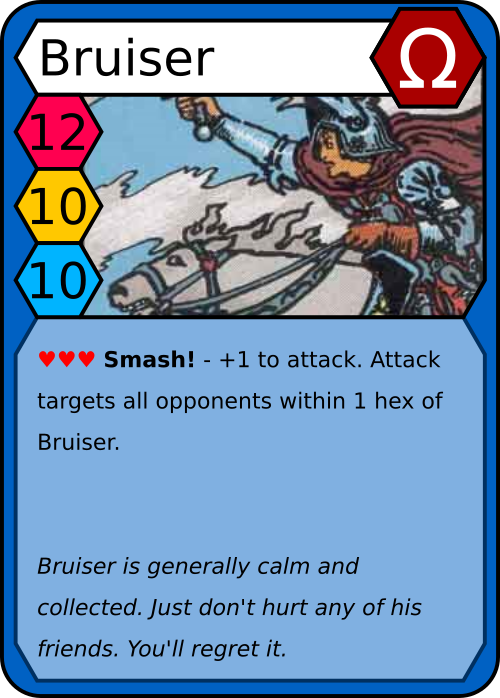
\includegraphics{graphics/bruiser-red.png}
    \caption{Special ability with associated Source cost.}
    \label{fig:ability-example}
\end{figure}

\figref{fig:ability-example} shows a character with a special ability called \textit{Smash!}.
Smash! requires three Hearts Source to be activated and provides the written bonus.

In addition to the special abilities written on each card, each team also has one or more special ability that applies universally to all characters on a team.

\begin{note} 
    Any number of abilities can be activated per turn, as long as there's enough Source to do so.
\end{note}
\subsection{Source}
Source is a special resource available to \textit{all} players in the game, which facilitates the activation of special abilities.
Each player may activate any number of special abilities on their own turn, as long as there's enough Source to do so.

\subsubsection{Source Types}
There are four different types of \textit{Source}, \textit{Hearts}, \textit{Spades}, \textit{Clubs}, \textit{Diamonds}\footnote{These are just for play-testing, and will be changed in the final version of the game}, as well as a fifth special type, \textit{Stars}.
Stars act as a wild-card and can consume any colour of Source.

\begin{figure}
    \centering
    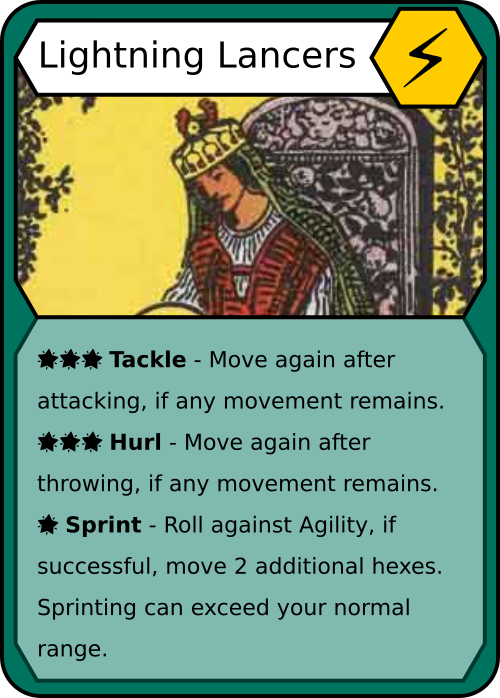
\includegraphics{graphics/yellow-team.png}
    \caption{Team card with wild-card Source abilities.}
    \label{fig:ability-example-2}
\end{figure}

\figref{fig:ability-example-2} shows a card that uses Stars as the ability cost.
Stars are considered colourless.
\subsubsection{Source Pool}
The Source Pool is the set of common Source cards available to all players, and is indicated by four or more face-up Source cards on the table.
To activate an ability discard the required number of Source cards of a given colour to consume them, then follow the ability's instructions as printed on the card.
Replenish the Source pool by drawing new cards, equal to the number of spent cards at the beginning of the next player's turn.

The number of Source cards increases every Third.
\subsubsection{Source Pool Size}
\begin{description}
    \item[1st Third] The Source pool contains 4 cards
    \item[2nd Third] The Source pool contains 6 cards
    \item[3rd Third] The Source pool contains 8 cards.
\end{description}